\section{Lecture 18: Checking \texorpdfstring{$!$}{!}-Covers --- Descendability, Closed and Open Covers, Zariski Descent}
\label{lec:18}

After the Christmas break, Clausen returns to the $!$-topology on the category
of affine analytic spaces $\Aff=(\AnRing)^{\mathrm{op}}$ set up in
\cref{lec:16,lec:17}. The plan of \cref{lec:17} left two goals; Goal~(1),
identifying presheaves that satisfy $!$-descent, was reached there. Today is
Goal~(2): how does one \emph{check} that a given map is a $!$-cover, and what are
the examples? The engine is a single proposition reducing $!$-descent to a
finitary condition on the unit object, refined in two directions (proper maps and
universally locally acyclic maps), from which closed covers, open covers, and
finally Zariski (and \'etale, fpqc, $h$-\dots) covers all fall out. The lecture
closes by re-running the same definitions inside ordinary algebraic geometry,
where they reproduce Mathew's notion of descendability. Throughout ``ring'' means
commutative ring and everything is (light) condensed.

\subsection{Recollection: the setup}
\label{subsec:18:recollection}

We recall the framework of \cref{lec:16,lec:17}. An analytic ring is a pair
\begin{equation}
\label{eq:18:anring}
R=(\ur R,\,D(R)),
\end{equation}
where $\ur R$ is a condensed animated ring and $D(R)\subseteq D(\ur R)=
\Mod_{\ur R}(D(\CondAbl))$ is a full subcategory of the (full, unbounded) derived
category of $\ur R$-modules, cut out by the completeness axioms
(\cref{def:8:analytic-ring,def:13:analytic-ring}); we take the whole $D(R)$, not
its connective part, as the primary invariant. The category of affine analytic
spaces is the opposite,
\begin{equation}
\label{eq:18:aff}
\Aff\ :=\ (\AnRing)^{\mathrm{op}}.
\end{equation}
Three classes of maps were singled out. For $f\colon X\to Y$ in $\Aff$ ---
equivalently a map of analytic rings $\ur R\to \ur S$ where $X=\AnSpec(S)$,
$Y=\AnSpec(R)$ --- one has the pullback $f^*\colon D(Y)\to D(X)$, and:

\begin{definition}[Proper maps and open immersions]
\label{def:18:proper-open}
\leavevmode
\begin{itemize}
\item $f$ is \emph{proper} if $f^*$ admits a \emph{good} right adjoint
$f_*$, where ``good'' means that $f_*$ commutes with base change (pullback),
commutes with colimits, and satisfies the projection formula. Equivalently, $X$
carries the \emph{induced} analytic ring structure from $Y$: $D(X)\subseteq D(\ur S)$ is
exactly the objects whose restriction of scalars to $D(\ur R)$ lies in $D(Y)$
(\cref{prop:16:proper-induced}). So the analytic ring structure is unchanged in
passing from $Y$ to $X$; only the underlying ring changes.
\item $f$ is an \emph{open immersion} if $f^*\colon D(Y)\to D(X)$ is a
localization (its right adjoint is fully faithful) and has a good left adjoint.
Equivalently, $f^*$ is localization away from an idempotent algebra $A\in D(Y)$
(``functions on the closed complement''), with
\begin{equation}
\label{eq:18:open-idempotent}
\ker\bigl(f^*\bigr)\ =\ \Mod_A\bigl(D(Y)\bigr).
\end{equation}
\end{itemize}
\end{definition}

\begin{definition}[$!$-able maps and $f_!$]
\label{def:18:shriekable}
A map $f\colon X\to Y$ is \emph{$!$-able} if it factors as an open immersion
followed by a proper map,
\begin{equation}
\label{eq:18:shriekable-factorization}
\begin{tikzcd}[column sep=large]
X \arrow[r, "j", hook] \arrow[rr, bend right=18, "f"'] & \overline X \arrow[r, "\pi"] & Y,
\end{tikzcd}
\end{equation}
$j$ an open immersion, $\pi$ proper. All three classes have good closure
properties: closed under composition and base change, containing all
isomorphisms, and closed under passage to diagonals (equivalently: given two
maps to a common target both in the class, any map between them lies in the
class). The six-functor formalism of \cref{lec:16} then produces $f_!$ exactly on
the $!$-able maps, with $f_!=f_*$ for $f$ proper and $j_!=$ the good left adjoint
of $j^*$ for $j$ an open immersion (equivalently $j^!=j^*$).
\end{definition}

\begin{remark}[The natural transformation $f_!\to f_*$]
\label{rmk:18:shriek-to-star}
There is a natural transformation $f_!\to f_*$ in general. For an open immersion it
comes from the natural map from the left adjoint of $j^*$ to its right adjoint,
present for any localization; one then composes and checks independence of the
factorization. A cleaner construction passes to the diagonal, using that the
diagonal of an open immersion is an isomorphism (as in ordinary algebraic
geometry).
\end{remark}

The descent condition and the topology it generates were the subject of
\cref{lec:17}.

\begin{definition}[$!$-cover]
\label{def:18:shriek-cover}
A $!$-able map $f\colon X\to Y$ is a \emph{$!$-cover} if the natural functor to the
totalization of the \v Cech nerve, formed with the \emph{upper-shriek} transition
functors, is an equivalence:
\begin{equation}
\label{eq:18:shriek-cover}
D(Y)\ \xrightarrow{\ \sim\ }\ \varprojlim_{n\in\Delta}{}^{!}\ D\bigl(X^{\times_Y n}\bigr).
\end{equation}
\end{definition}

\begin{theorem}[Equivalent forms, \cref{lec:17}]
\label{thm:18:tfae}
For $!$-able $f\colon X\to Y$, the following are equivalent.
\begin{enumerate}
\item $f$ is a $!$-cover.
\item \emph{($!$-codescent.)} The colimit, formed in $\PrL$ (equivalently in
$\Mod_{D(Y)}\PrL$) along the lower-shriek functors, recovers $D(Y)$:
\begin{equation}
\label{eq:18:codescent}
\varinjlim_{n\in\Delta^{\mathrm{op}}}\ D\bigl(X^{\times_Y n}\bigr)\ \xrightarrow{\ \sim\ }\ D(Y).
\end{equation}
\item \emph{($*$-descent with coefficients.)} For every $M\in\Mod_{D(Y)}\PrL$, the
$*$-pullbacks glue:
\begin{equation}
\label{eq:18:star-descent-coeff}
M\ \xrightarrow{\ \sim\ }\ \varprojlim_{n\in\Delta}{}^{*}\ M\otimes_{D(Y)}D\bigl(X^{\times_Y n}\bigr).
\end{equation}
\item \emph{($2$-descent.)} The assignment of module $\infty$-categories descends:
\begin{equation}
\label{eq:18:two-descent}
\Mod_{D(Y)}\PrL\ \xrightarrow{\ \sim\ }\ \varprojlim_{n\in\Delta}{}^{*}\ \Mod_{D(X^{\times_Y n})}\PrL.
\end{equation}
\end{enumerate}
Taking $M=D(Y)$ in (3) gives ordinary $*$-descent; so $!$-descent, a condition
about the exotic $(-)^!$-functors, upgrades to $*$-descent and even to descent one
categorical level up. Here $\Mod_{D(Y)}\PrL$ is the collection of presentable
$\infty$-categories tensored over the presentably symmetric monoidal
$\infty$-category $D(Y)$, with the naive relative-tensor base-change functors.
\end{theorem}

\begin{remark}[Finitary versus infinitary]
\label{rmk:18:finitary}
The topology is finitary by fiat: covers are finite families. One might instead
allow arbitrary (infinite) families and ask for $!$-descent. Scholze has checked
that this a priori infinitary version of the Grothendieck topology described below
is in fact finitary --- every cover admits a finite subcover. The point is that the
unit object $\mathbf 1_Y\in D(Y)$ is compact (\cref{prop:18:check}), so an
infinitary witness collapses to a finite stage. This is genuinely a feature of
\emph{$!$-descent}, not of $*$-descent: for $*$-descent alone one can have
infinitary covers of profinite sets with no finite subcover (e.g.\ a large
profinite set written as an infinite union of small ones), a phenomenon the set
theorists have examined. The universally submersive family of \emph{all} maps from
a fixed profinite set $P$ into the Cantor set is another candidate infinitary
cover whose cohomological (descent) behaviour is unclear.
\end{remark}

\subsection{Checking \texorpdfstring{$!$}{!}-covers: a finitary criterion}
\label{subsec:18:checking}

The following proposition reduces the (infinitary, $\infty$-categorical)
$!$-descent condition to a finitary membership statement, at the cost of an extra
hypothesis for its converse.

\begin{proposition}[Criterion for a $!$-cover]
\label{prop:18:check}
Let $f\colon X\to Y$ be a $!$-able map.
\begin{enumerate}
\item If $f$ is a $!$-cover, then the unit object lies in the thick subcategory
generated by the image of $f_!$:
\begin{equation}
\label{eq:18:unit-in-thick}
\mathbf 1_Y\ (=\mathcal O_Y)\ \in\ \bigl\langle\,\operatorname{im}\bigl(f_!\colon D(X)\to D(Y)\bigr)\,\bigr\rangle,
\end{equation}
where $\langle-\rangle$ denotes closure under the finitary operations: cones,
shifts, and retracts.
\item The converse holds provided \emph{either}
\begin{enumerate}
\item[\textup{(a)}] $f$ is proper; \emph{or}
\item[\textup{(b)}] $f$ is universally locally acyclic \textup{(U.L.A.)}, meaning
$f^!$ is good: it commutes with base change, commutes with colimits, and satisfies
the projection formula in the form
\begin{equation}
\label{eq:18:ULA}
f^!(-)\ \cong\ f^!(\mathbf 1_Y)\otimes f^*(-).
\end{equation}
\end{enumerate}
\end{enumerate}
\end{proposition}

\begin{remark}[The image of $f_!$ and compactness]
\label{rmk:18:image-thick}
Because $f_!$ is not fully faithful in general, its image has no closure
properties on its own; one must pass to the generated thick subcategory. One could
ask instead that $\mathbf 1_Y$ lie in the \emph{infinitary} (colimit-)closure of
the image; since $\mathbf 1_Y$ is compact in $D(Y)$, this is equivalent to the
finitary membership \eqref{eq:18:unit-in-thick}. Condition~(1) has the flavour of a
purely set-theoretic surjectivity of $f$ --- a ``cover'' condition, like a cover in
some constructible topology --- and by itself is much weaker than $!$-descent.
\end{remark}

\begin{remark}[The U.L.A.\ condition]
\label{rmk:18:ULA-meaning}
The object $f^!(\mathbf 1_Y)$ is the relative dualizing object of $f$. The good-ness
of $f^!$ is exactly the assertion that this dualizing object is compatible with
base change --- an equisingularity property of the family $X\to Y$. Properness and
U.L.A.\ are the analytic-geometry analogues of ``closed'' and ``open''
respectively (\cref{rmk:18:open-vs-closed}), and one may combine
\eqref{eq:18:unit-in-thick} with either to conclude honest descent; one cannot mix
open and closed, just as in topology finite closed covers and open covers each
give descent but a mixture need not.
\end{remark}

Part~(1) alone does not imply $!$-cover: the converse genuinely needs (a) or (b).

\begin{example}[The converse fails: an open glued to its closed complement]
\label{ex:18:converse-fails}
Take the induced solid structure on the affine line,
\begin{equation}
\label{eq:18:cex-Y}
Y=\AnSpec\bigl((\mathbb{Z}[T],\mathbb{Z})_\solid\bigr),
\end{equation}
and let $X=U\amalg Z$ be the disjoint union of the open piece and its closed
complement at infinity,
\begin{equation}
\label{eq:18:cex-X}
U=\AnSpec\bigl(\mathbb{Z}[T]_\solid\bigr)\xrightarrow{\ j\ }Y,\qquad
Z=\AnSpec\bigl(\mathbb{Z}(\!(T^{-1})\!)_\solid\bigr)\xrightarrow{\ i\ }Y,
\end{equation}
with $j$ an open immersion and $i$ a (proper) closed immersion. Here
\begin{equation}
\label{eq:18:cex-shrieks}
j_!\bigl(\mathbb{Z}[T]\bigr)=\operatorname{fib}\bigl(\mathbb{Z}[T]\to\mathbb{Z}(\!(T^{-1})\!)\bigr),
\qquad
i_!\bigl(\mathbb{Z}(\!(T^{-1})\!)\bigr)=\mathbb{Z}(\!(T^{-1})\!),
\end{equation}
the first being ``functions vanishing near infinity'' and the second $i_!=i_*$ the
forgetful functor. The unit $\mathbf 1_Y=\mathbb{Z}[T]$ is built from these two by
a single cofiber sequence
\begin{equation}
\label{eq:18:cex-cofiber}
j_!\,\mathbf 1_U\ \longrightarrow\ \mathbf 1_Y\ \longrightarrow\ i_*\,\mathbf 1_Z,
\qquad\text{i.e.}\quad
\operatorname{fib}\bigl(\mathbb{Z}[T]\to\mathbb{Z}(\!(T^{-1})\!)\bigr)\to \mathbb{Z}[T]\to\mathbb{Z}(\!(T^{-1})\!),
\end{equation}
so (allowing retracts) $\mathbf 1_Y$ lies in the thick subcategory generated by
$\operatorname{im}(f_!)$: \eqref{eq:18:unit-in-thick} holds. Yet $f=(j,i)$ is
\emph{not} a $!$-cover, because the descent object splits as $D(U)\times D(Z)$
rather than $D(Y)$ (the global sections on $U\amalg Z$ are the product ring). Here
$f$ mixes an open with a closed piece and is neither proper nor U.L.A., so neither
converse hypothesis applies.
\end{example}

\begin{proof}[Proof of \cref{prop:18:check}]
Spelling out \cref{def:18:shriek-cover}: the comparison functor
$D(Y)\to\varprojlim^!_{n}D(X^{\times_Y n})$ is a right adjoint (built from the
$(-)^!$ functors), and by general category theory it itself has a left adjoint,
informally
\begin{equation}
\label{eq:18:left-adjoint}
(M_n)_{n\in\Delta}\ \longmapsto\ \varinjlim_{n\in\Delta^{\mathrm{op}}} g_!\,M_n,
\end{equation}
where for each $n$ we write $g=g_n\colon X^{\times_Y n}\to Y$ for the structure
map. (Making this precise is due to Lurie.)

\emph{(1).} Full faithfulness of the comparison amounts to the counit
\begin{equation}
\label{eq:18:counit}
\varinjlim_{n\in\Delta^{\mathrm{op}}}\ g_!\,g^!\,M\ \xrightarrow{\ \sim\ }\ M
\end{equation}
being an isomorphism for all $M\in D(Y)$. Take $M=\mathbf 1_Y$. The geometric
realization \eqref{eq:18:counit} is a colimit over $\Delta^{\mathrm{op}}$, which one
filters by the partial totalizations
\begin{equation}
\label{eq:18:partial-tot}
\operatorname*{colim}_{n\in\Delta^{\mathrm{op}}_{\le d}}\ g_!\,g^!\,\mathbf 1_Y,
\end{equation}
each a \emph{finite} colimit (a nice fact about the simplex category: a partial
geometric realization is a finite colimit, expressible through iterated pushouts
and the initial object). Since $\mathbf 1_Y$ is \emph{compact}, an isomorphism
onto a filtered colimit factors through a finite stage: $\mathbf 1_Y$ is a retract
of some partial totalization \eqref{eq:18:partial-tot}. Every term there lies in
the image of $f_!$, since each structure map $g$ factors through $X\to Y$; and the
partial totalization is a finite colimit of such. Hence
$\mathbf 1_Y\in\langle\operatorname{im}(f_!)\rangle$.

\emph{(2).} Conversely, the hypothesis \eqref{eq:18:unit-in-thick} plus the
projection formula for $f_!$ gives that \emph{every} $M\in D(Y)$ is generated by
objects in the image of $f_!$: tensoring \eqref{eq:18:unit-in-thick} with $M$ and
using $f_!(f^*M\otimes N)\cong M\otimes f_!N$ shows $M\in\langle\operatorname{im}
f_!\rangle$ too. To prove the comparison is an equivalence we prove full
faithfulness and (separately) the other unit/counit. For full faithfulness we may,
by the previous sentence, assume $M=f_!N$; and we want the counit
\eqref{eq:18:counit} to be an isomorphism. The maps $g$ are composites of
pullbacks of $f$, so if $f$ has property (a) or (b), so does every $g$, and one has
a base-change identity commuting $g_!$ with $g^!$ (or $g'_!$ with $g'^!$ for the
various projections), by which one reduces to the split situation:
\begin{itemize}
\item \emph{proper case:} $g^!=g_*$ and base change follows from
$((-)^*,(-)_!)$-base change by passing to adjoints;
\item \emph{U.L.A.\ case:} $g^!=g^!(\mathbf 1)\otimes g^*$ and base change follows
directly from $((-)^*,(-)_!)$-base change.
\end{itemize}
(One must check the two a priori different base-change comparison maps agree, in
order to transport one being an isomorphism to the other.) This gives full
faithfulness. The remaining unit/counit is handled similarly, base-changing along
$X\to Y$, where the cover becomes split and the statement is formal.
\end{proof}

\subsection{Special cases: closed covers}
\label{subsec:18:closed}

We now make \cref{prop:18:check} concrete, beginning with the ``closed'' side.
Recall that $\Aff$ has proper maps and open immersions but no notion of closed
immersion was singled out; here is one.

\begin{definition}[Closed immersion]
\label{def:18:closed}
A map $f\colon X\to Y$ is a \emph{closed immersion} if it is proper and
$f^*\colon D(Y)\to D(X)$ is a localization. Since $f$ is proper, $D(X)=\Mod_{A}
D(Y)$ for the algebra $A:=f_*(\mathbf 1_X)\in D(Y)$; being a closed immersion is
then exactly the condition that $A$ be \emph{idempotent}, i.e.\ the multiplication
$A\otimes_{D(Y)}A\to A$ is an isomorphism.
\end{definition}

\begin{remark}[Open and closed are not complementary in $\Aff$]
\label{rmk:18:open-vs-closed}
In $\Aff$ it is not generally true that open and closed immersions with a fixed
target are in bijection: an open immersion need not have a closed complement in
$\Aff$, and a closed immersion need not have an open complement in $\Aff$.

Given an open immersion $j\colon U\to Y$ one gets an idempotent algebra $A\in D(Y)$
with $D(U)=D(Y)\,/\!\!/\,\Mod_A D(Y)$; but $A$ need not lie in $D_{\ge0}(Y)$, and
connectivity is exactly what is needed for $A$ to be the pushforward of an
\emph{animated} ring, hence to define a closed immersion in $\Aff$. For example,
with $Y=\AnSpec((\mathbb{Z}[X,Y],\mathbb{Z})_\solid)$ and
$U=\AnSpec(\mathbb{Z}[X,Y]_\solid)$, the corresponding idempotent $A$ has a nonzero
$H_{-1}$. (This is analogous to the scheme-theoretic phenomenon that the open
complement of a closed subscheme of an affine scheme need not be affine, though it
is still a scheme; here too one usually gets a closed complement that is an
analytic space, just not an affine one.)

In the other direction, given a closed immersion $Z\to Y$ --- an idempotent algebra
$A\in D_{\ge0}(Y)$ --- to obtain a complementary open \emph{in $\Aff$} one needs the
candidate localization functor
\begin{equation}
\label{eq:18:complement-open}
\underline{\RHom}_{D(Y)}\bigl(\operatorname{fib}(\mathbf 1_Y\to A),\,-\bigr)\colon\ D(Y)\to D(Y)
\end{equation}
to commute with filtered colimits and to preserve $D_{\ge0}(Y)$ --- precisely the
axioms making it define an analytic ring structure. These subtleties will be
largely fixed once one allows general (non-affine) analytic spaces and stacks.
\end{remark}

\begin{proposition}[Finite closed covers]
\label{prop:18:closed-cover}
Let $Z_1,\dots,Z_n\to X$ be closed immersions in $\Aff$ (with idempotent algebras
$A_i\in D_{\ge0}(X)$, so $Z_i\cap Z_j$ has algebra $A_i\otimes A_j$, etc.). Then
$\coprod_{i} Z_i\to X$ is a $!$-cover if and only if the structure sheaf satisfies
the most naive form of descent: the augmented \v Cech complex
\begin{equation}
\label{eq:18:closed-cech}
\mathbf 1_X\ \xrightarrow{\ \sim\ }\ \Bigl[\ \bigoplus_i \mathbf 1_{Z_i}\ \longrightarrow\ \bigoplus_{i<j}\mathbf 1_{Z_i\cap Z_j}\ \longrightarrow\ \cdots\ \Bigr]
\end{equation}
is an equivalence. The complex terminates at a finite stage.
\end{proposition}

\begin{proof}
If \eqref{eq:18:closed-cech} holds then $\mathbf 1_X$ lies in the image of the
lower-star ($=$ lower-shriek, as the $Z_i\hookrightarrow X$ are proper) functors
from the $\coprod Z_i$, so \cref{prop:18:check}(1) is met; and since the map is
proper, \cref{prop:18:check}(2a) upgrades this to a $!$-cover. Conversely, a
$!$-cover satisfies $*$-descent for $D(-)$, so $D(X)=\varprojlim$; plugging in the
unit object of $D(X)$ and reading off the base-change-then-right-adjoint yields
exactly the structure-sheaf descent \eqref{eq:18:closed-cech}.
\end{proof}

\subsection{Special cases: open covers}
\label{subsec:18:open}

Dually, for open immersions the criterion becomes vanishing of a product of the
complementary idempotents.

\begin{proposition}[Finite open covers]
\label{prop:18:open-cover}
Let $U_1,\dots,U_n\to X$ be open immersions, with complementary idempotent algebras
$A_1,\dots,A_n\in D(X)$ (so $A_i$ describes the closed complement of $U_i$). Then
\begin{equation}
\label{eq:18:open-criterion}
\coprod_i U_i\to X\ \text{ is a $!$-cover}\quad\Longleftrightarrow\quad A_1\otimes\cdots\otimes A_n=0\ \text{ in }D(X).
\end{equation}
Every open cover has a finite refinement, so no generality is lost in taking $n$
finite: the vanishing $A_1\otimes\cdots\otimes A_n=0$ of an algebra means
$\mathbf 1=0$ in it, and by compactness of the unit this is witnessed at a finite
stage.
\end{proposition}

Intuitively the $U_i$ cover $X$ precisely when the intersection of the
complementary closed sets is empty, i.e.\ $A_1\otimes\cdots\otimes A_n=0$.

\begin{proof}[Proof for $n=2$]
The general case reduces to $n=2$ by an induction using the appropriate
categorical form of the statement (the union $U_1\cup U_2$ need not itself lie in
$\Aff$). For $n=2$, $!$-descent for the cover is a Mayer--Vietoris pullback square
(the infinite \v Cech totalization collapses, as the $j$'s are monomorphisms),
\begin{equation}
\label{eq:18:MV-square}
\begin{tikzcd}[column sep=large, row sep=large]
D(X) \arrow[r, "j_1^!"] \arrow[d, "j_2^!"'] & D(U_1) \arrow[d, "j^!"] \\
D(U_2) \arrow[r, "j^!"'] & D(U_1\cap U_2),
\end{tikzcd}
\end{equation}
all maps upper-shriek. Reading off the induced statement for the unit object, this
is the assertion that $\mathbf 1_X$ is the total fiber of the Mayer--Vietoris
diagram of $j_{1,!}j_1^!\mathbf 1,\ j_{2,!}j_2^!\mathbf 1,\ j_{12,!}j_{12}^!\mathbf
1$; writing each $j_!j^!\mathbf 1$ in terms of the corresponding idempotent (recall
$j^!=j^*$ for an open immersion, and $j_!\mathbf 1=\operatorname{fib}(\mathbf 1\to
A)$), the cofiber sequence
\begin{equation}
\label{eq:18:MV-cofiber}
j_{12,!}\,j_{12}^!\,\mathbf 1\ \longrightarrow\ j_{1,!}\,j_1^!\,\mathbf 1\oplus j_{2,!}\,j_2^!\,\mathbf 1\ \longrightarrow\ \mathbf 1_X
\end{equation}
is directly equivalent, on unravelling, to $A_1\otimes A_2=0$. (Open immersions are
U.L.A., so \cref{prop:18:check}(2b) applies and the membership statement upgrades to
a genuine $!$-cover.)
\end{proof}

\subsection{Zariski (and \'etale, fpqc, \dots) covers}
\label{subsec:18:zariski}

We now produce genuine examples of $!$-covers by importing them from algebraic
geometry. There is a functor from ordinary commutative rings to analytic rings
sending $R$ (viewed as a discrete condensed ring) to the pair
\begin{equation}
\label{eq:18:cring-to-anring}
R\ \longmapsto\ \bigl(R,\,D^{\mathrm{cond}}(R)\bigr),
\end{equation}
where $D^{\mathrm{cond}}(R)$ is the full (large) derived category of \emph{all}
condensed $R$-modules --- no solidification is imposed. This works verbatim for
animated rings, and on opposite categories gives
\begin{equation}
\label{eq:18:affsch-to-aff}
\mathrm{AffDerSch}\ \longrightarrow\ \Aff,
\end{equation}
a functor commuting with finite limits (in particular sending the terminal object
to the terminal object): relative tensor products of animated rings go to relative
tensor products of analytic rings.

\begin{proposition}[Zariski descent]
\label{prop:18:zariski}
Under \eqref{eq:18:affsch-to-aff}, Zariski open covers of an affine (derived)
scheme go to $!$-covers.
\end{proposition}

\begin{proof}
A principal open $D(g)\subseteq\operatorname{Spec}R$, given by inverting $g$, goes
to a \emph{closed immersion} in $\Aff$: inverting $g$ produces an idempotent
algebra, and that algebra defines a closed cover in the sense of
\cref{prop:18:closed-cover}. The condition \eqref{eq:18:closed-cech} to be checked
is then just ordinary Zariski descent of the structure sheaf, which holds.
\end{proof}

\begin{remark}[Why Zariski opens look closed: the fuzz picture]
\label{rmk:18:fuzz}
That a Zariski open goes to a \emph{closed} immersion is Clausen's recurring
heuristic. In algebraic geometry one pictures the vanishing locus $\{f=0\}$ as
closed and the principal open $\{f\ne0\}$ as its open complement. But the
localization $R[1/f]$ does not literally delete $\{f=0\}$; derived-ly it deletes
the whole formal neighbourhood (the locus $\{f^n=0\}$ for all $n$), so the deleted
region acquires ``fuzz''. This fuzz makes the Zariski open behave like a
\emph{closed} subset with a boundary --- a tubular neighbourhood --- while the formal
neighbourhood that was removed plays the role of the open complement:
\begin{center}
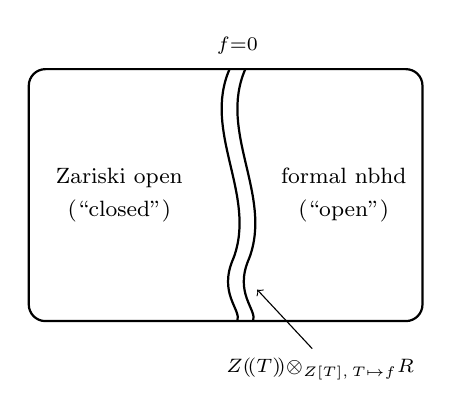
\begin{tikzpicture}[scale=1.0]
  \draw[thick, rounded corners=6pt] (0,0) rectangle (5,3.2);
  % fuzzy boundary curve
  \draw[thick] (2.55,3.2) .. controls (2.2,2.4) and (2.9,1.6) .. (2.6,0.8) .. controls (2.4,0.35) and (2.7,0.15) .. (2.65,0);
  \draw[thick] (2.75,3.2) .. controls (2.4,2.4) and (3.1,1.6) .. (2.8,0.8) .. controls (2.6,0.35) and (2.9,0.15) .. (2.85,0);
  \node at (2.65,3.5) {$\scriptstyle f=0$};
  \node[align=center] at (1.15,1.6) {\footnotesize Zariski open\\ \footnotesize (``closed'')};
  \node[align=center] at (4.0,1.6) {\footnotesize formal nbhd\\ \footnotesize (``open'')};
  \draw[->] (3.6,-0.35) -- (2.9,0.4);
  \node[anchor=north] at (3.7,-0.35) {$\scriptstyle \mathbb{Z}(\!(T)\!)\otimes_{\mathbb{Z}[T],\,T\mapsto f}R$};
\end{tikzpicture}
\end{center}
% Provenance: reconstructed from board 36--37 (00:35:34, 00:59--01:00, 01:30--01:33):
% a rectangle with a doubled (fuzzy) vertical boundary curve at the locus f=0,
% the left region labelled "Zariski open (closed)", the boundary curve labelled
% Z((T)) tensor_{Z[T], T->f} R.
Once one is in the solid world one can \emph{name} this boundary: base-change
$\mathbb{Z}(\!(T)\!)$ along $\mathbb{Z}[T]\to R$, $T\mapsto f$, to get an idempotent
algebra in $D\bigl((R[1/f])_{\mathbb{Z}_\solid}\bigr)$; removing this closed
boundary leaves an honest open, the complement
$D\bigl((R[1/f],\mathbb{Z}[1/f])_\solid\bigr)$. So there are two ways to embed
schemes into adic/analytic spaces:
\begin{equation}
\label{eq:18:two-embeddings}
R\ \longmapsto\ (R,\mathbb{Z})_\solid\qquad\text{and}\qquad R\ \longmapsto\ (R,R)_\solid.
\end{equation}
The first, base change to $\mathbb{Z}_\solid$, is the one above: Zariski opens look
closed. The second always removes the boundaries, and there Zariski opens go
genuinely to open immersions.
\end{remark}

\begin{remark}[The Grothendieck topology and the functor of topoi]
\label{rmk:18:topology-topoi}
One obtains a Grothendieck topology on $\Aff$ by declaring a sieve over $X\in\Aff$
to be a $!$-cover if it contains finitely many $!$-able maps $X_i\xrightarrow{f_i}X$
such that $\coprod_i X_i\xrightarrow{f}X$ is a $!$-cover in the sense of
\cref{def:18:shriek-cover}. That this defines a topology rests, beyond formal
properties of finite disjoint unions, on stability of $!$-covers under base change
--- itself a consequence of the $\PrL$-colimit description \eqref{eq:18:codescent},
since base change $\Mod_{D(Y)}\PrL\to\Mod_{D(Y')}\PrL$ commutes with colimits. In
particular one gets a functor
\begin{equation}
\label{eq:18:sheaves-functor}
\mathrm{Shv}_{\mathrm{Zar}}\bigl(\mathrm{AffDerSch};\mathrm{An}\bigr)\ \longrightarrow\ \mathrm{Shv}_{!}\bigl(\Aff;\mathrm{An}\bigr),
\end{equation}
which is in fact a pullback of topoi (it commutes with colimits and finite
limits). The target is essentially the category of analytic stacks, modulo two
technicalities deferred here: (i) one works with sheaves valued in anima
(homotopy types / Kan complexes / $\infty$-groupoids), and wants an intermediate
class of hyperdescent conditions strictly between plain-set descent and full
hyperdescent; (ii) the set-theoretic point that $\mathrm{CRing}$ is not small, so
one restricts to accessible presheaves and checks sheafification preserves
accessibility (cf.\ \cref{subsec:15:set-theory}).
\end{remark}

\begin{remark}[The topology is inexplicit]
\label{rmk:18:inexplicit}
More general covers descend as well; for instance \'etale covers give $!$-covers.
The essential difficulty going forward is that the $!$-topology is quite
inexplicit: unlike the Zariski or \'etale topologies, whose covers are finitely
generated with standard models, one has little a priori control over what a
$!$-cover can look like, so it is harder to rule out pathologies locally. Proving
full faithfulness of the passage from classical analytic geometries into analytic
stacks --- easy in the affine case at hand --- will in more complicated situations
require exactly the compactness/generation considerations of
\cref{prop:18:check}.
\end{remark}

\subsection{Appendix: relation to Mathew's descendability}
\label{subsec:18:descendability}

Much of this was motivated by Akhil Mathew's theory of \emph{descendability}
\cite{mathew2016galoisgroupstablehomotopy}. The discussion above is very
categorical, and one may re-run the same definitions inside ordinary algebraic
geometry: replace analytic rings by the pairs
\begin{equation}
\label{eq:18:disc-pair}
\bigl(R,\,D(R)\bigr),\qquad R\ \text{a (derived) commutative ring},\ D(R)\ \text{its usual derived category},
\end{equation}
so that $\Aff$ becomes affine (derived) schemes.

\begin{remark}[Everything is proper]
\label{rmk:18:everything-proper}
In this world a great simplification occurs: \emph{every} map is proper. Indeed for
$R\to S$ one has $D(S)=\Mod_S(D(R))$ almost by definition, which is the induced
structure. Hence every map is $!$-able. Beware that the resulting functors are not
the classical ones: $f^!$ is simply the right adjoint of $f_*$ (which exists for
general categorical reasons), \emph{not} the upper-shriek of Grothendieck duality.
For instance for $\pi\colon\operatorname{Spec}k[T]\to\operatorname{Spec}k$, the
functor $\pi^!$ here is not the Grothendieck-duality one, and $\pi_!=\pi_*$.
\end{remark}

\begin{proposition}[$!$-covers $=$ descendable maps]
\label{prop:18:descendable}
In the setting \eqref{eq:18:disc-pair}, a map $f\colon X\to Y$ is a $!$-cover if and
only if the unit lies in the thick subcategory generated by the image of $f_*$,
\begin{equation}
\label{eq:18:descendable}
\mathbf 1_Y\ \in\ \bigl\langle\, f_*\colon D(X)\to D(Y)\,\bigr\rangle,
\end{equation}
which is exactly Mathew's definition of \emph{descendability}. Consequently any
descendable map $R\to S$ (in Mathew's sense) gives a $!$-cover in $\Aff$ under the
functor \eqref{eq:18:affsch-to-aff}.
\end{proposition}

This holds because, every map being proper, \cref{prop:18:check}(2a) makes the
membership condition \eqref{eq:18:descendable} equivalent to being a $!$-cover.

\begin{example}[Descendable maps]
\label{ex:18:descendable}
Mathew gives many examples, all of which therefore yield $!$-covers:
\begin{itemize}
\item \'etale covers, and more generally \emph{countably presented} faithfully flat
maps $A\to B$ of ordinary rings (fpqc covers). The countable-presentation
hypothesis is apparently (probably genuinely) needed. For simplicial rings the
analogous condition should ask $\pi_0$ to be faithfully flat, with a further
condition on the higher $\pi_i$; Clausen did not work out the precise derived
statement.
\item $R\to R/I$ for $I$ a nilpotent ideal. Here descendability holds on the level
of \emph{derived} categories; it does \emph{not} say $D(R)=D(R/I)$, since the
descent is computed derived-ly and produces terms like $R/I\otimes^{\mathbb L}_R
D(-)$ in the colimit, not $R/I$ itself.
\item a proper surjective map of Noetherian schemes is descendable (extending the
affine discussion to schemes); and more generally any finitely presented
$h$-cover, combining the flat and proper cases.
\end{itemize}
By contrast $R\to\pi_0 R$ is not descendable in general: with $R=\mathbb{Q}[x]$,
$|x|=2$, inverting the degree-$2$ generator gives a ring module that vanishes
modulo $x$ but is nonzero. (The simplicial analogue of a nilpotent-ideal quotient
requires $R$ to be truncated --- finitely many homotopy groups, an Artinian-type
condition --- before $R\to\pi_0(R)/I$ becomes descendable.)
\end{example}

\begin{remark}[Independence of the ambient framework]
\label{rmk:18:framework-independent}
For a map of commutative rings one may ask whether descendability in ordinary
commutative algebra is equivalent to being a $!$-cover after applying
\eqref{eq:18:affsch-to-aff} into the condensed world. A priori the condensed side
could be a $!$-cover for some exotic reason involving condensed modules; but in fact
the two coincide. This uses a further characterization of descendability (Mathew):
one asks not merely for a limit diagram from the cosimplicial ring
$B,\ B\otimes_A B,\dots$, but for a \emph{uniformly} stable one --- the $n$-indexed
tower obtained from the cosimplicial object should be \emph{pro-isomorphic} to the
constant pro-object $A$ (so the vanishing is witnessed by a fixed finite shift at
every stage). This pro-object is the old discrete one, and the usual $D(R)$ embeds
fully faithfully into $D^{\mathrm{cond}}(R)$, hence
$\mathrm{Pro}(D(R))\hookrightarrow\mathrm{Pro}(D^{\mathrm{cond}}(R))$ fully
faithfully, so a pro-isomorphism upstairs is detected downstairs. (For the
pro-zero part one passes to fibers and may work in the homotopy category.)
\end{remark}

\begin{remark}[Mathew's general setting]
\label{rmk:18:mathew-general}
Mathew works in the generality of a presentably symmetric monoidal
$\infty$-category $\mathcal C\in\CAlg(\PrL)$ and an algebra object
$A\in\CAlg(\mathcal C)$, comparing $\mathcal C$ with $\Mod_A(\mathcal C)$:
\begin{equation}
\label{eq:18:mathew-setup}
\mathcal C\in\CAlg(\PrL),\quad A\in\CAlg(\mathcal C),\qquad \mathcal C\ \longrightarrow\ \Mod_A(\mathcal C).
\end{equation}
In our language every such map is proper, so his descendability is precisely the
proper-case of $!$-descent. This specializes to the condensed world, but only ever
addresses the proper maps, not the general $!$-able ones --- which is the extra
mileage of the present formalism.
\end{remark}

\begin{remark}[A decomposition formula, for perfect objects]
\label{rmk:18:decomposition}
In answer to a closing question: the ``decomposition formula'' from the previous
lecture\todo{Which formula from \cref{lec:17} is meant was left implicit in the
question (01:57:40); most likely the self-duality of $D(X)$ over $D(Y)$,
\cref{cor:17:self-dual}, or the associated finite resolution of the unit. Clausen
only confirmed the shape of the answer, not the precise object.} is not expected to
hold for all objects, but should hold for a suitable finiteness class such as the
perfect complexes, with a similar intuition. This kind of condition will resurface
when the six-functor formalism on $\Aff$ is extended to general analytic stacks,
where --- unlike the affine case settled today --- full faithfulness of the
comparison from classical analytic geometries is far from immediate.
\end{remark}
